\section{刚体的运动方程}\label{sec:10.4}

在第八章中,我们已经证明,对于任一质点系,其质心运动
都应满足下列方程
\begin{equation}\label{eqn:10.04.01}
  m \frac { \dif ^ { 2 } \vec{r} _ { c } } { \dif t ^ { 2 } } = \vec{F}
\end{equation}
当然,刚体也不例外。这时,式中$ m $是刚体质量,$ \vec{r} _ { c } $是刚体的质心
位置,$ \vec{F} $是刚体所受到的总外力。

在第九章中,我们已经证明,对一个质点,它的角动量$ \vec{l} $满
足下列的方程:
\begin{equation}\label{eqn:10.04.02}
  \frac { \dif \vec{l} } { \dif t } = \vec{M}
\end{equation}
其中$\vec{M}$是质点受到的力矩。对于刚体,我们可以定义它的角动量$ \vec{L} $
等于各质点的角动量之和,即

% 297.jpg
~\vspace{-2.56em}
\begin{equation}\label{eqn:10.04.03}
  \vec{L} = \sum_{ i = 1 } ^ n \vec{l} _ i
\end{equation}
这样,由式\eqref{eqn:10.04.02}可得
\begin{equation}\label{eqn:10.04.04}
  \frac { \dif \vec{L} } { \dif t } = \vec{M }
\end{equation}
\begin{align}\label{eqn:10.04.05}
  \beforetext{其中} \vec{M} = \sum_{ i = 1 } ^ n \vec{m} _ { i }
\end{align}
是刚体所受到的总外力矩。

\begin{wrapfigure}[9]{r}{12em}
  \vspace{-3em}
  \centering
  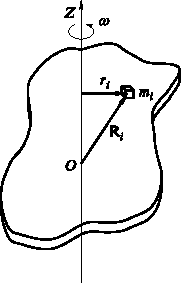
\includegraphics{figure/fig10.12}
  \caption{刚体围绕固定轴的转动}
  \label{fig:10.12}
\end{wrapfigure}
方程\eqref{eqn:10.04.01}及方程\eqref{eqn:10.04.04}合
在一起共有$ 6 $个独立的方程。因为刚体
只有$ 6 $个自由度,所以可以推测到,方
程\eqref{eqn:10.04.01}及方程\eqref{eqn:10.04.04}已经能够
描写刚体的全部的动力学。因此,它
们称为刚体的运动方程。

作为刚体运动方程的一个应用,
我们来讨论刚体绕一固定轴的转动。
如图\ref{fig:10.12},一刚体只能绕$ OZ $固定轴
转动,其角速度为$\omega$。为了确定整个
刚体的角动量$\vec{L}$,我们把刚体看成是由许多小块物质构成的。图
10.12中第$ i $小块对$ O $点的角动量为
\begin{equation*}
  \vec{l} _ { i } = m _ i \vec{R} _ i \times \vec{v} _ i
\end{equation*}
由于刚体只能绕$ OZ $轴转动,所以,我们只对$ \vec{l} _ i $在$ OZ $轴方向上的
分量有兴趣。这分量的大小是
\begin{equation*}
  m _ i r _ i v _i = m _ { i } r _ i ^ { 2 } \omega
\end{equation*}
其中$ r _ i $是第$ i $小块与轴$ OZ $的距离(\ref{fig:10.12})。在推导上式时,我们
已经用了关系式$ v _ i = r _ i \omega $。这样,刚体角动量$\vec{L}$沿$ OZ $轴的分量就
应等于\vspace{-0.8em}
\begin{equation}\label{eqn:10.04.06}
  L _ { z } = \Big( \sum_{ i = 1 } ^ { n } m _ { i } r _ i ^ { 2 } \Big) \omega = I \omega
\end{equation}

% 298.jpg
\noindent
其中$ I $是刚体对$ OZ $轴的转动惯量。

由此得到,绕定轴转动的刚体的基本方程是
\begin{equation}\label{eqn:10.04.07}
  \frac { \dif L _ { z } } { \dif t } = M _ { z }
\end{equation}
\begin{align}\label{eqn:10.04.08}
  \beforetext{或}\frac { \dif } { \dif t } \left( I \omega \right) = M _ { z }
\end{align}
其中$ M _ { z } $是力矩$\vec{M}$在$ OZ $方向的分量。

如果作用在刚体上的外力矩在$ OZ $轴方向的分量为零,则有
\begin{equation*}
  L_ { z } = \text{不变量}
\end{equation*}
即转动运动保持不变,刚体依靠“惯性”而永远转动;如果刚体
中物质的相对位置变化了,导致转动惯量从$ I _ 1 $变到$ I _ 2 $,则角速率
将从$ \omega _ 1 $变到$ \omega _ 2 $,并且
\begin{equation}\label{eqn:10.04.09}
  I _ { 1 } \omega _ { 1 } = I _ { 2 } \omega _ { 2 }
\end{equation}

\example 太阳绕自轴的旋转,其转速为每$ 22 $天一周,若坍缩
成中子星,试估计它的转速。

\solution 中子星中的物质可以简单地看成密排的中子,估计其密
度
$ \rho _ { n } = \dfrac { m _ { p } } { \dfrac { 4 \uppi } { 3 } r _ 0 ^ { 3 } } = \dfrac { 1 . 6 7 \times 1 0 ^ { - 2 7 } \text{ 公斤} } { \dfrac { 4 \uppi } { 3 } \left( 1 . 5 \times 1 0 ^ { - 15 } \text{ 米} \right) ^ { 3 } } = 1 . 1 8 \times 1 0 ^ { 1 7 } \text{ 公斤/米} $。已
知太阳质量 $ M _ { \text{日} } = 1 . 9 8 9 \times 1 0 ^ { 3 0 } \text{公斤} $,太阳半径 $ R _ {\text{日} } = 6 . 9 5 9 9 \times 1 0 ^ { 8 } \text{ 米} $,太阳若坍缩成中子星,则半径将变为$ R' $。它满足下面的关
系:
\begin{equation*}
  R ^ { \prime 3 } = \frac { M _ { \text{日} } } { \frac { 4 \uppi } { 3 } \rho _ { n } }= 4 . 0 2 4 \times 1 0 ^ { 1 2 } \text{ 米} ^ 3
\end{equation*}
\begin{align*}
  \beforetext{所以} R ^ { \prime } = 1 . 5 9 \times 1 0 ^ { 4 } \text{ 米}
\end{align*}
根据式\eqref{eqn:10.04.09},得

% 299.jpg
~\vspace{-1.5em}
\begin{equation*}
  \begin{split}
    \omega _ { 2 } &= \frac { I _ { 1 } } { I _ { 2 } } \omega _ { 1 } \\
    &= \frac { \dfrac { 2 } { 5 } M _ { \text {日} } R _ {\text{日}} ^2 } { \dfrac { 2 } { 5 } M _ { \text {日} } R ^ { \prime 2 } } \omega _ 1 \\
    &= \left( \frac { R _ { \text {日} } } { R ^ { \prime } } \right) ^ { 2 } \omega _ { 1 } \\
    &= \left( \frac { 6 . 9 5 9 9 \times 1 0 ^ { 8 } } { 1 . 5 9 \times 1 0 ^ { 4 } } \right) ^ { 2 } \times \frac { 2 \uppi } { 2 2 \times 2 4 \times 6 0 \times 6 0 } \\
    &= 6 . 3 3 \times 1 0 ^ { 8 } \text{ 弧度/秒}
  \end{split}
\end{equation*}
\begin{align*}
  \beforetext{或者} T _ { 2 } & = \left( \frac { R ^ { \prime } } { R _ { \text{日} } } \right) ^ { 2 } T _ { 1 }                                      \\
                            & = \left( \frac { 1 . 5 9 \times 1 0 ^ { 4 } } { 6 . 9 5 9 9 \times 1 0 ^ { 8 } } \right) ^ { 2 } \times 2 2 \text{ 天} \\
                            & = 1 . 1 5 \times 1 0 ^ { - 8 } \text{ 天}                                                                              \\
                            & \approx 0.99 \text{ 毫秒}
\end{align*}

由此得,若太阳坍缩成中子星,其转速是$ 0.99 $毫秒转一周。

下面我们讨论刚体运动中的外力作功的问题。为了表述简便,
我们讨论转动轴线虽不固定,但其方向不变(例如平行于$ Z $轴)的
情况。根据功的定义,有
\begin{equation*}
  A = T _ 2 - T _ 1
\end{equation*}
如果取质心为基点,动能可写为平动动能与转动动能之和,则上式
成为
\begin{align*}
  A & = \left( \frac { 1 } { 2 } m v _ { c 2 } ^ { 2 } + \frac { 1 } { 2 } I _ { c } \omega _ 2 ^ { 2 } \right) - \left( \frac { 1 } { 2 } m v _ { c 1 } ^ { 2 } + \frac { 1 } { 2 } I _ { c } \omega _ 1 ^ { 2 } \right) \\
    & = \left( \frac { 1 } { 2 } m v _ { c 2 } ^ { 2 } - \frac { 1 } { 2 } m v _ { c 1 } ^ { 2 } \right)
  + \left( \frac { 1 } { 2 } I _ { c } \omega _ 2 ^ { 2 } - \frac { 1 } { 2 } I _ { c } \omega _ 1 ^ { 2 } \right)
\end{align*}

由式\eqref{eqn:10.04.01}易证
\begin{equation*}
  \frac { 1 } { 2 } m v _ { c 2 } ^ { 2 } - \frac { 1 } { 2 } m v _ { c 1 } ^ { 2 } = \int _ { ( 1 \to 2 ) } \vec{F} \cdot \dif \vec{r} _ { c }
\end{equation*}
其中积分是沿着质心轨迹。又由式\eqref{eqn:10.04.08},并注意$ \omega = \dfrac { \dif \varphi } { \dif t } $,则
不难证明
\begin{equation*}
  \frac { 1 } { 2 } I _ { c } \omega _ 2 ^ { 2 } - \frac { 1 } { 2 } I _ { c } \omega _ 1 ^ { 2 } = \int _ {\varphi_{ 1 }} ^ {\varphi_{ 2 }} M \dif \varphi
\end{equation*}
\begin{align}\label{eqn:10.04.10}
  \beforetext{所以} A = \int _ { ( 1 \to 2 ) } \vec{F} \cdot \dif \vec{r} _ { c } + \int _ {\varphi_{ 1 }} ^ {\varphi_{ 2 }} M \dif \varphi
\end{align}
式中右边第一项是外力引起平动动能增加而作的功;第二项是外
力矩引起转动动能的增加而作的功。如果不取质心为基点,就不
能分解为平动和转动两项,我们再次看到质心作为基点的优越性。

由于式\eqref{eqn:10.04.10}对于$\vec{F}$及$ M $是线性的,所以,当刚体受到多个
外力的情况,第$ i $个外力$\vec{F}_i$及其力矩所作的功也类似可以写成为
\begin{equation}\label{eqn:10.04.11}
  A _ i = \int _ { ( 1 \to 2 ) } \vec{F} _ i \cdot \dif \vec{r} _ { c } + \int _ {\varphi_{ 1 }} ^ {\varphi_{ 2 }} M _ i \dif \varphi
\end{equation}

我们再次讨论车轮纯滚动问题,证明纯滚动过程中摩擦力并
不作功。在图\ref{fig:10.13} 中,我们画出摩擦力$\vec{F}$。由式\eqref{eqn:10.04.11},摩擦力
对刚体所作的功为
\begin{equation*}
  \begin{split}
    A &= \int \vec{ F } \cdot \dif \vec{r} + \int M \dif \varphi \\
    &= \int F \dif x + \int \left( - F r _ { 0 } \right) \dif \varphi \\
    &= F \Delta x + \left( - F r _ { 0 } \Delta \varphi \right) \\% 301.jpg
    &= F \left( \Delta x - r _ { 0 } \Delta \varphi \right)
  \end{split}
\end{equation*}

\clearpage
\begin{figure}[h]
  \centering
  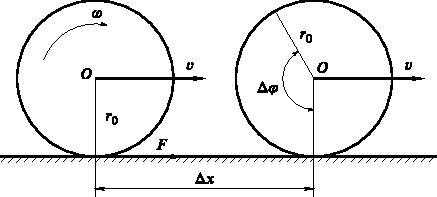
\includegraphics{figure/fig10.13}
  \caption{纯滚动中的摩擦力不作功}
  \label{fig:10.13}
\end{figure}
式中力矩$ M = F r _ { 0 } $取负号,是因为它使车轮绕质心的转动方向与$ \varphi $
增加的方向相反。又因是纯滚动,故有
\begin{equation*}
  \Delta x - r _ { 0 } \Delta \varphi = 0
\end{equation*}
最后得到
\begin{equation*}
  A = 0
\end{equation*}

需要指出,尽管刚体问题纯粹是牛顿力学的问题,但与质点
问题有很大的不同,它的基本运动方程是式\eqref{eqn:10.04.01}、\eqref{eqn:10.04.04}。
又如所谓刚体处于平衡状态,是指其质心加速度为零,同时角动
量不变的状态,因此刚体的平衡条件为
\begin{equation}\label{eqn:10.04.12}
  \begin{cases}
    \vec{ F } & = 0 \\
    \vec{ M } & = 0
  \end{cases}
\end{equation}

除此之外,在处理理想刚体(即无形变,可以不考虑滚动摩
擦)的纯滚动问题时,滚动物与其它物体的接触点处相对速度为
零,在此点若有摩擦力存在,是为静摩擦力,判断该静摩擦力的
方向需要十分小心。这里有一个一般可用的原则:设想此物与接
触点脱离,使摩擦不复存在,此时触点切向加速度的反方向,即
为静摩擦力的方向。

下面看几个实例:

恒力$\vec{ F }$作用在半径为$ r $的匀质小球$ m $的球心$ C $处,使小球在
% 302.jpg
地面上作纯滚动,如图\ref{fig:10.14} 所示。设想$ O $点脱离接触,摩擦力不
再存在,由于$\vec{ F }$通过质心,小球无转动或转动状态不变,$ O $点的切
线加速度即为质心的加速度,方向向右。因此,静摩擦力$ \vec{f} $的方
向应当向左(图\ref{fig:10.14})。

若开始时,小球以$ \omega_{ 0 } $角速度, $ \vec{v} _ { 0c } $ 的质心速度在水平地面上作
纯滚动,然后力$\vec{F}$作用在质心$ C $上,如图\ref{fig:10.15} 所示。设想摩擦力
不存在,由于$\vec{ F }$通过质心,对于质心没有力矩,所以$ O $点的切向加
速度即为质心$ C $的加速度,方向向左。因此,静摩擦力$\vec{f}$的方向应
当向右,与$\vec{F}$反向。

\begin{figure}[h]
  \begin{minipage}{0.5\linewidth}
    \centering
    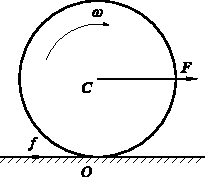
\includegraphics{figure/fig10.14}
    \caption{}
    \label{fig:10.14}
  \end{minipage}
  \begin{minipage}{0.5\linewidth}
    \centering
    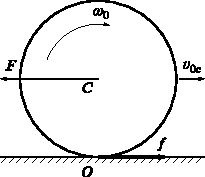
\includegraphics{figure/fig10.15}
    \caption{}
    \label{fig:10.15}
  \end{minipage}
\end{figure}

现有一半径为$ r $,质量为$ m $的小球在粗糙的半圆形碗底作纯滚
动,此时小球质心受到切向外力,其大小为$ | \vec{F} _ t | = m g \sin \theta $, $ \vec{F} _ t $ 总
是指向平衡位置$ O $,如图\ref{fig:10.16} 所示。根据前面的判断方法,$\vec{f}$总是
与$ \vec{F} _ t $反向,并总是背向平衡点$ O $;在小球位于平衡点时, $ \vec{f} = 0 $。

\begin{figure}[h]
  \centering
  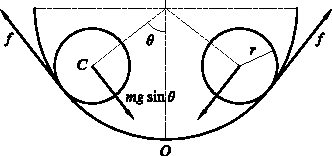
\includegraphics{figure/fig10.16}
  \caption{}
  \label{fig:10.16}
\end{figure}

% 303.jpg
\clearpage
\example 有一匀质圆柱,重$ 200 $公斤,如果加上一通过其质
\begin{wrapfigure}[6]{r}{11em}
  \centering
  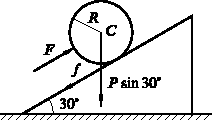
\includegraphics{figure/fig10.17}
  \caption{}
  \label{fig:10.17}
\end{wrapfigure}
心、与$ 30^\circ $倾角的固定斜面相平行、方向朝
上的$ 150 $公斤力,使其向上作无滑动
的纯滚动(如图\ref{fig:10.17})。试求圆柱体质
心的线性加速度以及斜面与圆柱间的
摩擦力。

\solution 圆柱的质心在重力、摩擦力
$\vec{f}$及外加力$ \vec{F}=150 $公斤作用下作加速运动,$\vec{f}$的方向根据上面的讨
论可以确定如图\ref{fig:10.17} 所示。整个圆柱又在力矩$ fR $作用下绕通过
质心的轴作加速转动,故有方程
\begin{equation*}
  \begin{split}
    F - P \sin 3 0 ^ { \circ } - f &= \frac { P } { g } a _ { c } \\
    f R &= I \beta \\
    &= \frac { 1 } { 2 } \cdot \frac { P } { g } R ^ { 2 } \beta
  \end{split}
\end{equation*}
另有约束条件
\begin{equation*}
  a _ { c } = R \beta
\end{equation*}
解之得
\begin{equation*}
  \begin{split}
    a _ { c } &= \frac { 1 } { 6 } g \\
    &= 1 6 3 . 3 \text{厘米/秒} ^ 2 \\
    f &= 1 6 . 7 \text{公斤力}
  \end{split}
\end{equation*}

一般来说,如果外力不是作用在质心上,或外力的作用线不
通过质心,此时静摩擦力的方向不但与外力的方向有关,而且与
力的作用线至转轴的垂直距离有关。

\example 设小球在力$ \vec{F} $作用下在平直地面上作纯滚动,$ \vec{F} $不是
作用在质心$ C $上,而是作用在$ O' $上,$ O' $是接触点$ O $与
质心连
\clearpage\noindent
线上的
一点, $ C O ^ { \prime } = d $,如图\ref{fig:10.18} 所示。设小球半径为$ r $,质
量为$ m $。试
% 304.jpg
判断接触点$ O $处静摩擦力的方向。

\begin{wrapfigure}[8]{r}{11em}
  \centering
  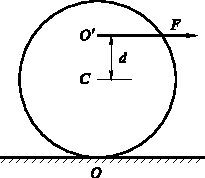
\includegraphics{figure/fig10.18}
  \caption{}
  \label{fig:10.18}
\end{wrapfigure}
\solution 设$ O $点没有摩擦力,则绕质
心的转动公式为
\begin{equation*}
  \begin{split}
    F d &= I \beta \\
    I &= \frac { 2 } { 5 } m r ^ { 2 }
  \end{split}
\end{equation*}
质心的运动方程为
\begin{equation*}
  \vec{a} _ { c } = \frac { \vec{F} } { m }
\end{equation*}
触点$ O $对地面的切向加速度$ \vec{a} $的大小为
\begin{equation*}
  \begin{split}
    a &= a _ { c } - \beta r \\
    &= \frac { F } { m } \left( 1 - \frac { 5 d } { 2 r } \right)
  \end{split}
\end{equation*}
由此可得以下判断:

(1) 当 $ d < \dfrac { 2 } { 5 } r $ 时, $ a > 0 $ ,即$ \vec{a} $与$ \vec{F} $同向,所以静摩擦力$ \vec{f} $与
$ \vec{F} $反向;

(2) 当$ d > \dfrac { 2 } { 5 } r $时, $ a < 0 $ ,$ \vec{a} $与$ \vec{F} $反向,则$ \vec{f} $与$ \vec{F} $同向;

(3) 当$ d = \dfrac { 2 } { 5 } r $时, $ a = 0 $ ,此时$ O $点无运动的趋向,则$ \vec{f} = 0 $;

(4) 特别当外力$ F=0 $时,则$ \vec{a} $恒为零,$ \vec{f} $恒为零,小球将
保持匀速纯滚动。

\example 拉线轴问题。在水平的粗糙桌面上放一外半径为
$ R $,质量为$ m $的线轴,以力$ \vec{F} $拉线,拉线处距轴中心距为$ r $,如图
\ref{fig:10.19} 所示。改变$ \theta $角能否使线轴向前(即顺$ \vec{F} $前方)无滑动地滚
动?

\solution 先判定$ \vec{f} $的方向。设若$ \vec{f} $不存在,则得方程

\clearpage
\begingroup
\mathindent=2em
\begin{equation*}
  \begin{split}
    F \cos \theta &= m a _ c \\
    F r &= - I _ { c } \beta
  \end{split}
\end{equation*}
\begin{wrapfigure}[11]{r}{13em}
  \vspace{-4em}
  \centering
  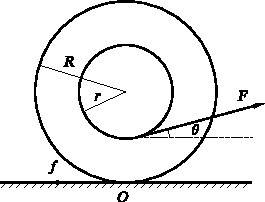
\includegraphics{figure/fig10.19}
  \caption{}
  \label{fig:10.19}
\end{wrapfigure}
(在此,顺钟向为$ \beta $正方向。\!\!) $~ O $
点的切向加速度为
\begin{equation*}
  \begin{split}
    a _ { 0 } &= a _ { c } + \beta R \\
    &= F \left( \frac { \cos \theta } { m } + R \frac { r } { I _ { c } } \right)
  \end{split}
\end{equation*}
\endgroup
在$ \theta < 90 ^ \circ $情况F,$ a _ 0 $恒大于零,\\
即与$ \vec{F} $同方向。所以$\vec{f}$与$\vec{F}$反向,如图\ref{fig:10.19} 所示。

进一步列出线轴纯滚动方程:
\begin{equation*}
  \begin{split}
    F \cos \theta - f &= m a _ { c } \\
    f R - F r &= I _ { c } \beta \\
    a _ { c } &= R \beta
  \end{split}
\end{equation*}
解此联立方程,得
\begin{equation*}
  a _ { c } = \frac { R F \left( R \cos \theta - r \right) } { I _ { c } + m R ^ { 2 } }
\end{equation*}
从上式可以得出:

$ \theta < \cos ^ { - 1 } \left( \dfrac { r } { R } \right) $ 时, $ a _ { c } > 0 $ ,轴向前滚动;

$ \theta > \cos ^ { - 1 } \left( \dfrac { r } { R } \right) $
时, $ a _ { c } < 0 $ ,轴向后滚动;

$ \theta = \cos ^ { - 1 } \left( \dfrac { r } { R } \right) $
时, $ a _ { c } = 0 $ ,轴不动。

\noindent
$ \theta _ { 0 } = \cos ^ { - 1 } \left( \dfrac { r } { R } \right) $
是一个临界值,当$ \theta = \theta_{ 0 } $时,$ \vec{F} $的作用线恰好通过
接触点$ O $,$\vec{F}$对$ O $点的力矩为零;当$ \theta < \theta_{ 0 } $时,$ \vec{F} $对$ O $点的力矩
的方向使线轴向前作纯滚动;当$ \theta > \theta _ { 0 } $时,$\vec{F}$对$ O $点的力矩的方向
使线轴向后作纯滚动。

% 306.jpg
\clearpage
\example 汽车主动轮的运动情况,类似于车轮受力偶的作
用,如图\ref{fig:10.20} 所示。

\begin{wrapfigure}[7]{r}{13em}
  \vspace{-1.56em}
  \centering
  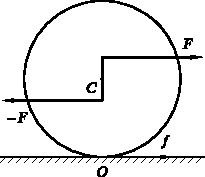
\includegraphics{figure/fig10.20}
  \caption{}
  \label{fig:10.20}
\end{wrapfigure}
设想$ O $点脱离接触,则$ O $点
的切向加速度即为力偶作用下绕
$ C $点的切向加速度,方向向左,
所以$ O $点的静摩擦力$\vec{f}$的方向向
右,如图\ref{fig:10.20} 所示。

在某些情况下,刚体并非作
纯滚动,而是既有滚动,又有滑
动,我们称它为“连滚带滑”的运动。此时接触点与接触面之间
的相对速度不为零,刚体受到的是滑动摩擦力。
